\chapter{Theoretischer Hintergrund}
\label{chap:theoretischer-hintergrund}
Zum Architekturprinzip der Microservices gibt es bereits eine Vielzahl akademischer Publikationen.
In diesem Kapitel wird in den theoretischen Hintergrund der für diese Thesis relevanten Literatur eingeführt.
Zunächst wird ein kurzer Vergleich zwischen dem häufig verwendeten Legacy-Architekturprinzip \emph{Monolith} und dem behandelten neuen Architekturprinzip \emph{Microservices} gezogen.
Anschließend werden aktuelle Arbeiten zur Migration zu Microservices-Architekturen beschrieben.
Des Weiteren wird das \acrfull{mmf} vorgestellt, das ein wesentlicher Bestandteil und Untersuchungsobjekt dieser Arbeit ist.
Abschließend wird ein Überblick über das Produkt gegeben, das mithilfe des \gls{mmf} überarbeitet werden soll.

\section{Vergleich von monolithischen und Microservices-Systemen}
\label{sec:monolith-vs-microservices}

Die monolithische Systemarchitektur hat lange Zeit einen Großteil der Softwareprodukte ausgemacht und ist die konventionelle Art, Software zu entwickeln.
Moderne Programmiersprachen ermöglichen zwar die Modularisierung von Monolithen, jedoch befindet sich die gesamte Funktionalität eines Monolithen in einer Applikation, die aus nur einem ausführbaren Artefakt besteht.
Nach den meisten Definitionen (siehe~\cite{Dragoni2017}) sind Monolithen dadurch gekennzeichnet, dass ihre einzelnen Module nicht unabhängig voneinander ausführbar sind.
Auch wenn in dieser Arbeit die Migration weg von dieser Architektur thematisiert wird, hat sie ihre Vorteile.
Da es sich um eine simple Architektur mit nur einer Codebasis handelt, ist das Erstellen, Testen, Deployment und auch Monitoring kleiner Anwendungen einfacher und schneller~\cite{a-survey-on}.
Es ist kein kompliziertes Kommunikationsmodell notwendig, da Monolithen oft in einer Programmiersprache und sogar mit nur einem Framework geschrieben werden.

Je größer Monolithen jedoch werden, desto stärker zeigen sich die Schwächen dieser Architektur.
Es entstehen riesige Codebasen und kleine Änderungen erzwingen erneutes Bauen und Testen der gesamten Applikation~\cite{Dragoni2017}.
Dies steht auch im Widerspruch zu modernen agilen Arbeitsprinzipien.
Wenn nur einzelne Komponenten eines Monolithen eine hohe Last erfahren, muss trotzdem das gesamte System skaliert werden, was zu einer Verschwendung von Rechenleistung führen kann und die Anwendung ineffizient macht~\cite{Dragoni2017}.
Außerdem kann schnell das Problem der \qq{Dependency Hell}~\cite{Dragoni2017} auftreten, wobei das Hinzufügen oder Ändern von Abhängigkeiten dazu führen kann, dass das gesamte Projekt nicht mehr kompiliert oder ausgeführt werden kann.

Die meisten dieser Probleme werden durch die Microservices-Architektur gelöst.
Dabei besteht ein System aus vielen kleinen (Micro-) Services.
Diese zeichnen sich dadurch aus, dass sie möglichst klein gehalten werden, genau eine Aufgabe haben und unabhängig ausgeführt werden können~\cite{a-survey-on}.
Durch die Entkopplung der Services wird im Gegensatz zu Monolithen ein Kommunikationsmodell zwischen den Services notwendig.
Dafür existieren verschiedene Lösungen, die im Rahmen dieser Arbeit näher betrachtet werden.
Eine sehr häufig eingesetzte Lösung ist beispielsweise \gls{rest}.

Die Vorteile dieser Architektur gegenüber Monolithen sind vielseitig.
Da die Services unabhängig voneinander konzipiert sind, können sie einzeln implementiert, getestet und gebaut werden.
Dies erleichtert die Automatisierung des Bauens und Testens durch \gls{ci}/\gls{cd}.
Es ermöglicht auch, dass die Anwendung während eines Updates auf eine neue Version durchgehend online bleibt~\cite{a-survey-on}.
Des Weiteren können Services abhängig von der Last einzeln skaliert werden, was die Effizienz in bestimmten Szenarien deutlich erhöht.
Darüber hinaus sind Entwickler flexibel in der Wahl der Programmiersprache und des Frameworks für einzelne Services, da die einzige Anforderung die Umsetzung des gewählten Kommunikationsmodells ist.

Eine Microservices-Architektur ist allerdings nicht universell einer monolithischen Architektur vorzuziehen.
Gründe dafür sind einige Nachteile von Microservices-Architekturen, die von \Citet{a-survey-on} zusammengetragen wurden.
Dazu gehört vor allem die Komplexität des Systems, die bei einer Microservices-Architektur deutlich höher ist.
Dies liegt an der Aufteilung des Systems in einzelne Services und der nichttrivialen Kommunikation zwischen den Services.
Viele Entwickler müssen die neue Architektur mit ihrer erhöhten Komplexität, sowie die zugehörigen Werkzeuge und Mechanismen für automatisierte Tests, Deployments und Monitoring erst erlernen.
Der resultierende Netzwerk-Overhead durch die Kommunikation zwischen den Komponenten kann zu höheren Latenzen führen und das System ineffizient machen, wohingegen bei Monolithen lediglich Funktionen innerhalb desselben laufenden Programms aufgerufen werden.
Des Weiteren ist es empfehlenswert, dass Microservices jeweils eigene Datenbanken haben.
Das fügt weitere Komplexität zum Design hinzu, da Daten dupliziert werden müssen und die Konsistenz der Datenbanken gewährleistet sein sollte.
All dies führt dazu, dass Experten empfehlen, für kleine Anwendungen bei monolithischen Architekturen zu bleiben~\cite{a-survey-on,7742218}.

\section{Migration zu Microservices}

Aufgrund der beschriebenen Vorteile von Microservices Architekturen ist es im Interesse vieler Unternehmen und Entwickler, existierende Applikationen und Systeme mit monolithischer Architektur zu Microservices-basierten Systemen zu migrieren.
Der Planungsprozess dieser Migration ist allerdings sehr zeit- und kostenintensiv und durch große Risiken geprägt, da dabei Systeme tiefliegend verändert werden.
Deswegen ist die Migration zu Microservices seit etwa 2015 ein stark untersuchtes Thema.

Bei der Migration zu Microservices gibt es mehrere zentrale Herausforderungen, die jedes Entwicklerteam bewältigen muss und auch in der \hyperref[forschungsfrage:1]{Forschungsfrage} als Untersuchungsobjekt dieser Thesis genannt werden.
Eine der größten ist die Dekomposition des vorhandenen, großen, zusammenhängendem Systems in kleine, unabhängige Services~\cite{a-survey-on,taibi2017processmotivations,taibi2019decomposition}.
Die sogenannte optimale Granularität der Services zu bestimmen, ist eine sehr wichtige Aufgabe, da sie starke Auswirkungen auf die Performanz des Systems haben kann.
Der Nachteil zur großer Services ist, dass sie ineffizient werden und womöglich ähnliche unerwünschte Eigenschaften erhalten wie monolithische Systeme.
Dagegen ist auch eine Aufteilung in zu kleine einzelne Einheiten problematisch, da dadurch der Kommunikationsbedarf zwischen den Microservices stark erhöht werden kann, was ebenfalls leistungsbezogene Nachteile hat.
Für diesen entscheidenden Prozess wäre es also wichtig für Entwicklerteams, wissenschaftlich gestützte Entscheidungen treffen zu können.
%Die existierenden Werkzeuge für die Dekomposition bieten allerdings nur beschränkte Funktionalität über statische Code- oder Abhängigkeiten-Analyse~\cite{a-survey-on}.
%Deswegen gibt es einige literarische Vorschläge für Frameworks zur Dekomposition~\cite{taibi2019decomposition,taibi2019monolithic}.

Ebenfalls ist die Konzipierung der Inter-Service Kommunikation ein wichtiger Bestandteil, der starke leistungsbezogene Auswirkungen haben kann.
Das liegt daran, dass im Vergleich zu monolithischen Systemen die Kommunikation zwischen den Services die Latenz für gleichartige Aufgaben erhöht.
Um diesen Effekt zu minimieren, sollte möglichst wissenschaftlich gestützt vorgegangen werden und Best Practices sowie beliebte Pattern evaluiert und verwendet werden.

Bei der Migration zu Microservices gibt es neben den zwei genannten viele andere Her\-aus\-for\-de\-run\-gen, wie Mangel an Verständnis, Identifikation der Service-Grenzen, Testing, Fehlertoleranz, Serviceintegration, Datenkonsistenz, hohes Coupling im Legacy-System, organisatorische Her\-aus\-for\-de\-run\-gen, Sicherheit, Datenbank-Migration, Datenmanagement und Monitoring \cite{migration-challanges2023}.
Um diese verschiedenen Her\-aus\-for\-de\-run\-gen nicht einzeln angehen zu müssen, kann ein Framework hilfreich sein, das den gesamten Refactoring-Prozess in mehreren Phasen begleitet.
Ein solches wird im nächsten Kapitel vorgestellt und anschließend in dieser Arbeit untersucht.

\section{\acrfull{mmf}}
\label{sec:mmf}

Es wurden bereits viele Gründe für die sehr häufig durchgeführte Migration zu Microservices, sowie die Risiken und Herausforderungen dabei beschrieben.
Dass der Migrationsprozess sehr komplex, risikoreich und fehleranfällig ist, sollte klar sein.
Erschwert wird er durch das Fehlen klarer und strukturierter Anleitungen.
Mehrere Metastudien haben bereits versucht, eine Übersicht über verschiedene Refactoring- und Migrationsverfahren zu geben, die für Entwickler hilfreich sein können.
Jedoch bleibt dabei das Problem bestehen, dass sich der aktuelle Stand der Literatur schnell ändert und Metastudien dadurch teilweise obsolet werden.
Dieses Problem könnte durch die Umsetzung der Anleitung in Form eines Werkzeugs, das Entwickler bei der Migration unterstützt, gelöst werden.
Im Gegensatz zu Metastudien könnte dieses Werkzeug dynamisch an den neuesten Forschungsstand angepasst werden.

Aus diesem Grund hat das \gls{ese} das \acrfull{mmf} und das zugehörige Werkzeug \gls{arh} \cite{arh-github} entwickelt, welche in diesem Kapitel vorgestellt werden.
Während \Citet{fritzsch2022architecturecentric} den Entwurf des Frameworks für das Werkzeug beschreiben, wurde das Werkzeug im Rahmen von zwei Masterarbeiten entwickelt \cite{master-daniel-koch,master-tobias-haller} und in einer ersten Fallstudie angewendet \cite{master-marvin-knodel}.
Der \gls{arh} ist eine web-basierte Anleitung, die Entwickler durch drei Phasen der Migrationsplanung führt.
Eine Übersicht über diese Phasen und die Funktionsweise des Frameworks ist in \cref{fig:mmf-overview} zu sehen.
Im Folgenden werden diese drei Phasen genauer beschrieben:

\begin{itemize}
	\item \textbf{Phase 1: System Comprehension:}
	In Phase 1 wird das Verständnis des Systems, das migriert werden soll, angestrebt.
	Mit den Stakeholdern sollen dabei strategische Ziele für Produkt und Unternehmen definiert, sowie \glspl{qa} und gewünschte Szenarien identifiziert werden.
	Es sollen sich dadurch mögliche Treiber für die neue Microservices-Architektur herauskristallisieren.
	Durch das resultierende Verständnis des Systems wird ein Vergleich der alten monolithischen Architektur und einer potentiellen neuen Microservices-Architektur möglich.
	Architekten sollen dann mithilfe dieser Informationen eine Entscheidung für oder gegen die Migration zu Microservices fällen.
	Im Werkzeug ist in dieser Phase bisher nur die Eingabe der Szenarien mit zugehörigen \glspl{qa} in der Arbeit von \Citet{master-daniel-koch} umgesetzt worden.
	\item \textbf{Phase 2: Strategy Definition:}
	Falls sich in Phase 1 für die Migration zu Microservices entschieden wurde, wird in Phase 2 die Planung der Migration begonnen.
	Die hauptsächliche Aufgabe in dieser Phase ist die Entscheidung, welche Migrationsstrategie benutzt werden soll, um das System zu modernisieren.
	Dafür kann zwischen (momentan) 115 verschiedenen Methoden gewählt werden, die aus akademischen Publikationen stammen.
	Das Werkzeug kann Entwickler dabei unterstützen, indem es basierend auf Eingaben aus Phase 1 empfohlene Methoden vorschlägt.
	Einige dieser Methoden beinhalten die Nutzung von Werkzeugen, welche auch gesondert durchsucht werden können.
	Die verschiedenen Migrationsmethoden und Werkzeuge können von Admins importiert, exportiert und bearbeitet werden, wodurch die Erweiterung in zukünftigen Arbeiten vereinfacht möglich ist.
	\item \textbf{Phase 3a: Architecture Definition:}
	Phase 3 ist in zwei Teile aufgeteilt.
	Im ersten Abschnitt wird die neue Architektur definiert.
	Hier wird, basierend auf der Methode zur Migration, die in der Planungsphase gewählt wurde, der \gls{sia} durchgeführt.
	Außerdem wird allgemeiner die Architektur des gesamten Systems geplant, wobei das Werkzeug Entwickler durch eine Liste von vorgeschlagenen Patterns und Best Practices unterstützen kann.
	 Phase 3a und 3b sind eng verbunden, denn durch Erkenntnisse in der Implementierung kann die Planung häufig noch mehrmals überarbeitet werden und dadurch eine neue Implementierung begonnen werden.
	\item \textbf{Phase 3b: Service Implementation:} In Phase 3b startet dann ein Zyklus von Im\-ple\-men\-tie\-rung\-en der in Phase 3a definierten Services.
	Bei Implementierung selbst kann das Werkzeug Entwickler nicht unterstützen.
	Doch Bestandteil der Entwicklungszyklen ist auch, dass das entstehende System anhand der Qualitätsmerkmale zu bewerten.
	Dadurch kann eine unpassende Architekturdefinition oder auch eine unpassende Aufteilung in Services frühzeitig erkannt und korrigiert werden.
	Ist diese Phase abgeschlossen, ist eine erste Version des migrierten Systems fertig.
\end{itemize}

\begin{figure}
	\centering
	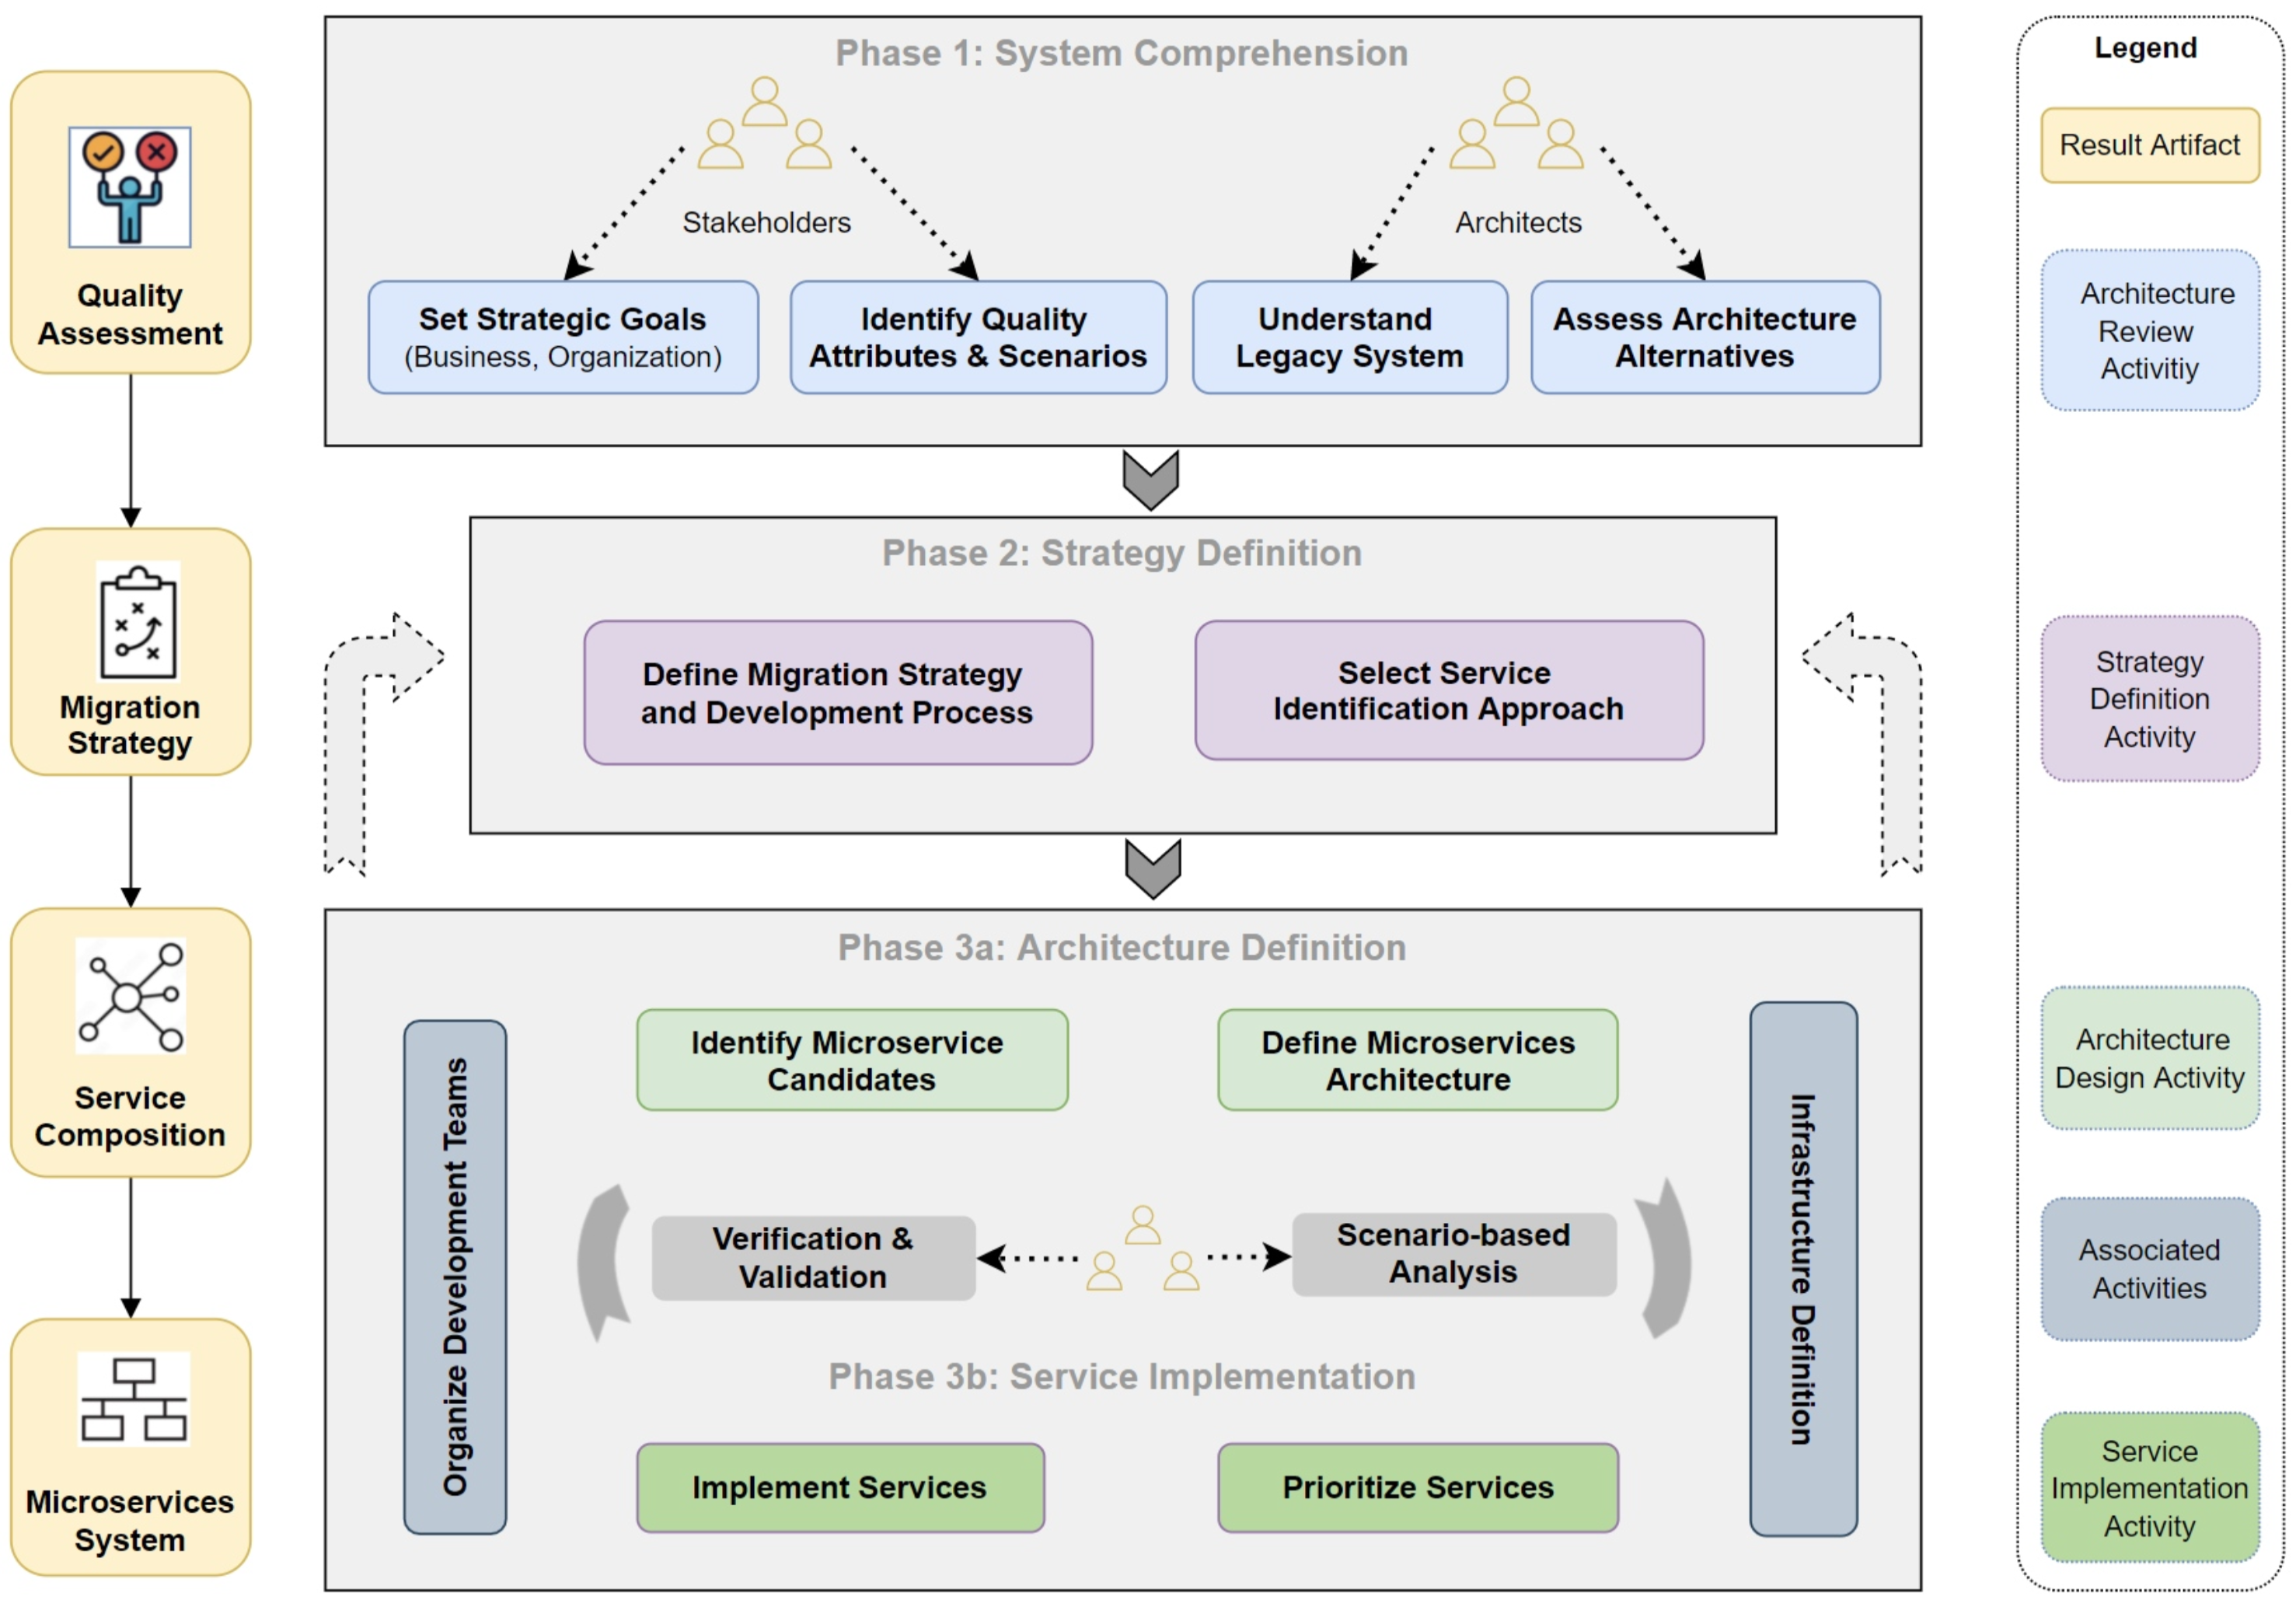
\includegraphics[width=\textwidth]{mmf-overview}
	\caption[\acrfull{mmf} Übersicht]{
		Übersicht über das \gls{mmf} des \gls{ese} \cite{fritzsch2022architecturecentric}. Es sind die drei Phasen des Prozesses zu erkennen, sowie einige Schritte der einzelnen Phasen.
	}
	\label{fig:mmf-overview}
\end{figure}

\section{jadice flow}

Das vorgestellte Framework soll in dieser Thesis nun erstmals zum Refactoring einer bereits vorhanden Microservices-Architektur in der Industrie benutzt werden.
Deswegen wird in diesem Abschnitt näher auf das Produkt \emph{jadice flow}\footnote{\url{https://flow.jadice.com/}} eingegangen, welches mit dem \gls{mmf} überarbeitet werden soll.

\emph{jadice flow} ist ein Produkt der Firma \emph{levigo solutions}\footnote{\url{https://solutions.levigo.de/}}.
\emph{levigo solutions} beschäftigt über 30 Mitarbeiter, von denen ungefähr sechs seit vier Jahren an \emph{jadice flow} arbeiten.
\emph{jadice flow} basiert bereits auf einer Microservices-Architektur, ist jedoch erst die erste Generation nach der Überführung des vorherigen Monoliths \emph{jadice server}\footnote{\url{https://jadice.com/produkte/server/}}.
Beide Produkte bieten Workflow-basierte Dokumentenverarbeitung an, bei der mit komplexen Datenströmen umgegangen werden kann.
Durch den Umstieg auf eine Microservices-Architektur können in der neuen Generation einzelne Verarbeitungsschritte skaliert werden.
Der Großteil der Services ist in Java geschrieben, doch durch den Betrieb in Containern ist \emph{jadice flow} prinzipiell unabhängig von der Programmiersprache.

Einen beispielhaften Workflow stellt der \emph{E-Mail converter} dar.
Dabei werden E-Mails in Einzelteile aufgeteilt (Körper, Anhänge) und diese dann einzeln in das Zielformat konvertiert.
Die einzelnen Arbeitsschritte dabei können parallelisiert und separat skaliert werden.
Am Ende werden die Ergebnisse kombiniert.
Im Gegensatz zu einfacher PDF-Darstellung von E-Mails in geläufigen Programmen bietet \emph{jadice flow} zusätzliche Features, wie die tiefe Analyse und Darstellung von Archiven in Anhängen.

Da \emph{jadice flow} die erste Generation in Microservices-Architektur ist, wird noch architektonisches Verbesserungspotential vermutet.
Durch die Analyse von \emph{jadice flow 1.0} mithilfe des Werkzeugs und weiterer Forschung im Rahmen dieser Bachelorarbeit soll ein Refactoring-Prozess für \emph{jadice flow 2.0} angestoßen werden.

Obwohl das Framework für die Anwendung auf Monolithen gedacht ist, soll in dieser Arbeit die Anwendung des Frameworks auf ein bereits migriertes System angewendet werden, um dessen Eigenschaften weiter zu verbessern.
Dadurch wird erforscht, inwiefern sich Framework und Werkzeug auf eine bereits existierende Microservice-Architektur anwenden lassen.
Falls es deshalb für diesen Anwendungsfall zielführend ist, wird zusätzlich die ursprüngliche monolithische Anwendung von \emph{jadice flow} (\emph{jadice server}) hinzugezogen.
Die Ergebnisse dessen könnten dann mit \emph{jadice flow} verglichen werden.

\section{Ähnliche Forschung}

Aufgrund vieler Vorteile von Microservices vor allem direkt gegenüber traditionellen Monolithen (ausführlicher im \cref{sec:monolith-vs-microservices} diskutiert) ist die Migration zu Microservices zu einem großen Forschungsfeld geworden.
In diesem Abschnitt wird ein Überblick über für diese Arbeit relevante Publikationen gegeben.

\subsection{Grundlagen zum \gls{mmf}}

Das Hauptuntersuchungsobjekt dieser Thesis sind das \gls{mmf} und der \gls{arh} des \gls{ese}.
Obwohl das Werkzeug sich noch in einer prototypischen Phase befindet, wurde es bereits durch mehrere akademische Publikationen weiterentwickelt.
Im Folgenden wird ein Überblick über diese gegeben.
Im Jahr 2019 kategorisierten \Citet{10.1007/978-3-030-06019-0_10} zehn verschiedene Microservices-Migrationsmethoden.
Dabei wird ein Mangel an praktisch anwendbaren Methoden hervorgehoben, die gute Werkzeugunterstützung und Metriken zur Verifikation der Ergebnisse bieten.
Als Folge darauf stellten \Citet{fritzsch2022architecturecentric} die Planung eines solchen Frameworks vor.
Der Migrationsprozess mit Framework und dessen Arbeitsweise in drei Phasen wird beschrieben.
Außerdem wird die Entwicklung eines Werkzeugs erwähnt, das das Framework in Form einer Web-basierten Lösung umsetzt und Entwickler bei der Migration unterstützt.
Die Entwicklung des Werkzeugs fand im Rahmen der Masterarbeiten von \Citet{master-tobias-haller} und \Citet{master-daniel-koch} statt.
\citeauthor{master-tobias-haller} forscht dabei an der erweiterbaren Speicherung von verschiedenen Migrationsmethoden und der Darstellung dieser in der Web-Applikation, dem \gls{arh}.
Damit wurde größtenteils das Backend und Phase 2 des Werkzeugs umgesetzt.
Schlussendlich wird außerdem eine empirische Bewertung des entstandenen Prototyps vorgenommen, die den Nutzen des Werkzeugs bestätigt und weiterführende Arbeit daran vorschlägt.
\Citet{master-daniel-koch} setzt die Arbeit an dem Werkzeug fort, indem Phase 1 und 3 ergänzt werden.
Dabei wird viel an \glspl{qa} in der Migration zu Microservices geforscht.
Zu Beginn werden relevante \glspl{qa} gesammelt, wobei ein Großteil davon aus ISO 25010~\cite{ISO-25010} stammt, welche durch weitere, oft Microservices-kontextuelle \glspl{qa}, ergänzt werden.
Außerdem wird der Einfluss der \glspl{qa} auf Systemeigenschaften untersucht.
Sehr relevant für den \gls{arh} ist ebenfalls die durchgeführte Untersuchung, wie durch den Nutzer definierte \glspl{qa} den Vorschlag passender Migrationsmethoden in Phase 2, sowie profitabler Design Patterns und Best Practices in Phase 3 unterstützen kann.

In 2023 führt \citeauthor{master-marvin-knodel} im Rahmen einer Masterarbeit \cite{master-marvin-knodel} eine erste Fallstudie zur Anwendung des \gls{mmf} durch.
Dabei wird das Framework im Ganzen als geeignet für die Migration im Einzelfall der Fallstudie bestätigt.
Außerdem werden kleinere Mängel hervorgehoben, die weitere Arbeit am Framework und Tool nahelegen.
Diese Fallstudie unterscheidet sich von der in dieser Arbeit durchgeführten Fallstudie in einigen Punkten.
Zum einen bilden die Arbeiten verschiedene Anwendungsfälle ab.
Während in \Citet{master-marvin-knodel} der vermutlich gewöhnlichere Fall vorliegt, bei dem ein Monolith zu einer \gls{msa} umstrukturiert werden soll, fügt diese Arbeit einen neuen Anwendungsfall hinzu.
Die Evaluierung und Verbesserung einer bereits vorhandenen \gls{msa} erfordert möglicherweise andere Qualitäten des Frameworks, insbesondere bei der gezielten Suche nach Verfahren, die für diesen speziellen Fall überhaupt anwendbar sind.
Zum anderen steht eine weiter ausgeprägte Version des Werkzeugs \gls{arh} zur Verfügung.
Während die Suche nach Migrationsverfahren von in der Arbeit von \citeauthor{master-marvin-knodel} manuell ausgeführt wurde \cite{master-marvin-knodel}, kann zum Zeitpunkt dieser Arbeit die Suchfunktion des \gls{arh} dafür genutzt werden.

\subsection{Andere Frameworks}
%\subsection{Andere Frameworks mit Tool-Support}

Im Gegensatz zu den im nächsten Abschnitt behandelten Refactoringverfahren, die in großer Zahl akademisch publiziert wurden, liegt nur sehr wenig Forschung zu Verfahren auf der Metaebene vor \cite{on-a-metaprocess}.
Das Funktionsprinzip des \gls{mmf} ist dabei bisher einzigartig.
Wie auch \Citet{master-marvin-knodel} beschreibt, ist kein Framework bekannt, das den Vergleich und die Suche über viele konkrete Migrationsverfahren aus der Metaebene anbietet und damit direkt mit dem \gls{mmf} vergleichbar ist.
Es existieren nur wenige andere Frameworks, die im Gegensatz zu spezifischen Migrationsverfahren ebenfalls in der Metaebene Migrationsprozesse anleiten.
Jene sollen unter diesem Aspekt mit dem \gls{mmf} in Relation gesetzt werden.
%In diesem Abschnitt werden ähnliche Frameworks und Werkzeuge beschrieben, die Entwickler aus einer Meta-Perspektive bei der Migration unterstützen, wie es auch \gls{mmf}, beziehungsweise \gls{arh} machen.

\Citet{on-a-metaprocess} stellen die Methode \gls{m3k} vor, die auf dem OMG Essence Kernel~\cite{essence-kernel-omg} basiert.
Dieses Werkzeug soll Ent\-wick\-ler\-teams beim Migrationvorgang helfen, indem ein allgemeiner Metaprozess definiert wird, der als Grundlage für spezifische Migrationsprozesse verwendet werden kann.
Die Evaluation von \gls{m3k} steht noch aus, Fallstudien und Expertenumfragen sind jedoch geplant.
Im Gegensatz zum \gls{mmf} liefert \gls{m3k} lediglich eine generische Prozessübersicht.
Verweise auf konkrete Methoden, um die einzelnen Schritte jedes Teils des Migrationsprozesses umzusetzen, sind dabei nicht vorhanden.
Nutzer werden dadurch bei der Umsetzung der identifizierten Schritte weniger unterstützt als beim \gls{mmf}.

%\Citet{software-architectural-migration-2021} stellen eine automatisierten Ansatz vor, mit dem Ar\-chi\-tek\-tur\-mi\-gra\-ti\-on\-en geplant werden können und der mehrere Zielarchitekturen neben Microservices unterstützt.
%Er basiert auf der formalen Modellierung der strukturellen und verhaltensbezogenen Aspekte der Architektur.
%Anhand dieser Eingaben werden Teile des Designs identifiziert, die überarbeitet werden sollten, wodurch eine neue Zielarchitektur bestimmt wird.
%Diese kann mit einer \emph{model-checking} Technologie formal gegenüber den funktionalen Anforderungen validiert werden.
%Mit einer KI-Planungstechnik werden einzelne Schritte für die Migration zur Zielarchitektur entworfen.
%Für diese Schritte können inkrementell vorläufige Modelle bestimmt werden, sowie formal überprüft werden, ob diese Modelle mit den definierten funktionalen und architektonischen Bedingungen übereinstimmen.
%Dieser Ansatz wurde mit fünf Architekturen von echten Software Systemen getestet, wobei unter anderem das Refactoring zu einer Microservices-Architektur erfolgreich war.
%In Zukunft soll die Liste der unterstützten Zielarchitekturen erweitert werden, sowie Unterstützung auf Implementierungs-Level hinzugefügt werden.

%In einem weiteren Artikel stellen \Citet{architect:a-framework} das Framework \emph{Architect} vor.
%Sie beschreiben, wie sie das System \emph{Artemis} mithilfe des Frameworks in zwei Phasen in eine Microservices-Architektur modernisieren.
%Während in der ersten Phase die Dekomposition des Systems durchgeführt wird, findet in der zweiten Phase die Trennung der geteilten Datenbank in mehrere Datenbanken nach \emph{database-per-microservice} Pattern statt.
%\emph{Architect} ist allerdings noch relativ limitiert, da es nur Projekte von Grund auf unterstützt, also keine Unterstützung für Software-Evolution bietet, nur dotnet-basierte Services erstellt und nur relationale Datenbanken unterstützt.

\subsection{Konkrete Refactoring-/Migrationsverfahren}
%\subsection{Konkrete Refactoring-/Migrationsverfahren mit Tool-Support}

Im Gegensatz zu dem, was in dieser Arbeit bisher als \emph{Frameworks} bezeichnet wurde, werden in diesem Abschnitt konkrete Refactoring-Verfahren betrachtet.
Diese sind durch die Vorgabe einer spezifischen Strategie klar von Meta-Ansätzen wie dem \gls{mmf} abzugrenzen.
Der \gls{arh} speichert momentan 115 solcher Verfahren.
Ein wichtiges Feature des \gls{mmf} und \gls{arh} ist dabei die Kategorisierung dieser Verfahren, die eine individuelle Suche für verschiedene Nutzer des Frameworks mit unterschiedlichen Zielen ermöglicht.
Um einen Überblick über die Merkmale zu geben, in denen sich Methoden unterscheiden, werden folgend einige in akademischen Publikationen beschriebene Verfahren vorgestellt.

Eines der primären Merkmale ist das Ziel eines Verfahrens.
Die meisten Verfahren behandeln das Ziel, eine geeignete Dekomposition von Monolithen in Microservices zu finden, da dies eines der kompliziertesten Probleme bei der Migration darstellt.
Jene Verfahren sind für diese Thesis besonders relevant, da in der Forschungsfrage gezielt danach gesucht wird.
Beispiele für Methoden, die dieses Ziel verfolgen, sind \cite{arh-result-no-filter-3,arh-result-no-filter-2,arh-result-no-filter-5,arh-result-important-filter-4,arh-result-important-filter-7}.
Es gibt jedoch auch wenige andere Verfahren, die andere Ziele haben.
Dazu gehören die Prognose der Nützlichkeit einer potenziellen \gls{msa} für Systeme vor der Migration \cite{muP-a-dev-framework}, die Bewertung und Analyse von Schwachpunkten nach einer Migration \cite{https://doi.org/10.1002/spe.2974} oder die reine technische Umsetzung einer Dekomposition unter Angabe der erwünschten Service-Aufteilung \cite{arh-result-no-filter-4}.

Die für diese Thesis relevante Kategorie der Methoden, die der Dekomposition eines Monolithen dienen, kann anhand weiterer Merkmale unterteilt werden.
Dies umfasst hauptsächlich Merkmale, die die Funktionsweise der Verfahren betreffen.
Eine erste Unterscheidung kann bezüglich der Form der Eingabe in die Methoden gemacht werden.
Während einige mit Source-Code oder Laufzeit-Artefakten arbeiten und darauf statische und dynamische Analysen ausführen \cite{arh-result-no-filter-5}, erwarten andere Eingaben auf \acrlong{bp} Ebene \cite{arh-result-no-filter-3} oder \emph{User Stories} \cite{arh-result-no-filter-2}.

Die meisten Verfahren erstellen dann aufgrund dieser Eingaben einen Graphen mit unterschiedlichen atomaren Einheiten als Knoten (abhängig von der Eingabe).
Anschließend wird bei verschiedenen Methoden mit unterschiedlichen Algorithmen versucht, eine bestmögliche Gruppierung in dem Graph zu finden.
Viele Verfahren verwenden unterschiedliche Versionen von \emph{Clustering}-Algorithmen \cite{arh-result-no-filter-3,arh-result-no-filter-5,arh-result-important-filter-4}, andere lösen das Problem mit evolutionären beziehungsweise genetischen Algorithmen \cite{arh-result-no-filter-2,arh-result-important-filter-7}.

Unter anderem abhängig von den Eingabemöglichkeiten gibt es verschiedene Stufen der Au\-to\-ma\-ti\-sie\-rung.
Vor allem Verfahren, die mit Code-Analysen arbeiten, sind teilweise voll-automatisiert \cite{Fil2023}.
Für andere Eingabearten wie \acrfull{bp} oder \emph{User Stories} ist höchsten semi-Automatisierung möglich, da diese Eingaben manuell erstellt werden müssen.
Die algorithmische Optimierung eines erzeugten Graphen ist in der Regel theoretisch automatisch möglich.
Allerdings ist dies nicht immer umgesetzt oder es wird lediglich auf mögliche Algorithmen für die Umsetzung verwiesen.


%Die wohl häufigste Art von Methoden sind solche, die Entwickler bei der Dekomposition von Monolithen in Microservices unterstützen.
%%Der \gls{arh} speichert momentan 20 dieser Werkzeuge.
%Jeder dieser Ansätze setzt unterschiedliche Bedingungen für die Anwendung voraus.
%Es gibt einige voll-automatische Werkzeuge, die zwar im Bezug auf die Eingabe unflexibler sind und damit nicht in jedem Fall anwendbar, aber eine einfachere und schnellere Anwendung ermöglichen.
%Auf der anderen Seite gibt es auch semi-automatische Werkzeuge, bei denen Entwickler oft über Formulare oder Graphen ihr System beschreiben müssen, da der Code nicht direkt analysiert werden kann.
%Dies bietet allerdings den Vorteil von höherer Kompatibilität.
%Im Folgenden werden zwei Bespiele für solche Werkzeuge vorgestellt.

%\Citet{Fil2023} stellen ein voll automatisiertes Migrationswerkzeug vor.
%Dieses arbeitet mit statischer Code-Analyse, um eine Graph-Repräsentation des monolithischen Systems zu erhalten.
%Ein solcher Graph dient als Ausgangslage für weitere automatische Analysen, die in mehreren Schritten eine Dekomposition in Services durchführen und diese weiter optimieren.
%Schlussendlich soll das Ergebnis eine Menge von hochgradig kohäsiven und lose gekoppelten Microservices sein.
%Dabei soll eine angemessene Granularität der Microservices erreicht werden.
%Die ebenfalls durchgeführte Evaluation ergibt positive Ergebnisse im Bezug auf Effektivität und Effizienz des Werkzeugs.
%Sie ist allerdings nur begrenzt valide, da nur wenige und kleine Monolithen als Eingabe für das Experiment fungiert haben.

%\Citet{PF4MD} stellen das semi-automatische Werkzeug \emph{PF4MD} vor, das Entwicklern bei der Dekomposition eines Monolithen in Microservices unterstützen soll.
%Sie beschreiben eine Ähnlichkeit der Microservices Architektur und der \gls{pf} nach \Citet{problem-frames} im Bezug auf das Aufteilen komplexer Probleme in kleinere, besser handlichere Teile.
%Aufgrund dieser Ähnlichkeit wollen sie das Problem der Dekomposition in Microservices mit der Beschreibung des Systems in graphisch umgesetzten Problem Diagrammen lösen, die auf \gls{pf} basieren.
%Mithilfe der eingegebenen Problem Diagramme und weiterer Eingaben, die die Problemkomplexität sowie die strukturelle Komplexität verschiedener Probleme quantifizieren, kann das Werkzeug eine Aufteilung der Probleme in verschiedene Gruppen vorschlagen.
%Eine Evaluation des Werkzeugs oder dieser Methode wurde bisher nicht durchgeführt.

%Eine weitere Art von Werkzeugen sind Werkzeuge für den Post-Migrationszeitraum.
%Diese unterstützen natürlich nicht die Migration, da diese schon abgeschlossen ist, sondern führen eine Bewertung des Ergebnisses durch und analysieren Schwachpunkte.
%Ein Beispiel zeigt der Artikel zur $\mu$TOSCA toolchain.
%\Citet{https://doi.org/10.1002/spe.2974} beschreiben, wie sie mit dem  $\mu$TOSCA Modell Architekturen von Microservices-basierten Systemen mit dem OASIS Standard TOSCA darstellen können.
%Außerdem beschreiben sie die Möglichkeit, das $\mu$TOSCA Modell eines Systems durch das zugehörige Kubernetes Deployment automatisch zu ermitteln.
%Das $\mu$TOSCA Modell einer Applikation soll dann dazu genutzt werden, potentielle architektonische Probleme zu finden.
%Für das Ermitteln des $\mu$TOSCA Modells und das Identifizieren von Architektur Smells stellen sie zwei Werkzeug Prototypen ($\mu$Miner und $\mu$Freshener) vor.

%Die letzte in dieser Arbeit behandelte Art von Werkzeugen sind Werkzeuge, die vor der Migration angewendet werden.
%Diese werden oft zur Prognose über eine mögliche Migration benutzt.
%Ein Beispiel dafür ist das von \Citet{muP-a-dev-framework} vorgeschlagene Framework $\mu P$.
%Dieses soll die Performance einer hypothetischen Microservices-Architektur durch das Design abschätzen können und dadurch Entwickler bei der Entscheidung unterstützen, ob sich eine Migration zu Microservices lohnt.
%Basierend auf vier Benchmarks wurde das Framework getestet, wobei der Fehler der Antwortzeiten konstant unter 10\% lag.
